\documentclass[tikz,border=10pt]{standalone}
\usepackage{tikz}
\usepackage{amsmath,amssymb}
\usetikzlibrary{shapes,arrows,positioning,fit,calc,decorations.pathreplacing}
\usepackage{xcolor}

% Define colors matching the original
\definecolor{inputblue}{RGB}{135,206,250}
\definecolor{rfblue}{RGB}{65,105,225}
\definecolor{probgreen}{RGB}{144,238,144}
\definecolor{thresholdgray}{RGB}{192,192,192}
\definecolor{benigngreen}{RGB}{34,139,34}
\definecolor{maliciousred}{RGB}{220,20,60}
\definecolor{lightgray}{RGB}{245,245,245}

\tikzset{
    inputbox/.style={rectangle, rounded corners=8pt, minimum width=3cm, minimum height=1.2cm, text centered, draw=black, fill=inputblue},
    rfbox/.style={rectangle, rounded corners=8pt, minimum width=2.5cm, minimum height=1cm, text centered, draw=black, fill=rfblue, text=white},
    probbox/.style={rectangle, rounded corners=5pt, minimum width=1.5cm, minimum height=0.8cm, text centered, draw=black, fill=probgreen},
    threshbox/.style={rectangle, rounded corners=5pt, minimum width=2cm, minimum height=1.2cm, text centered, draw=black, fill=thresholdgray},
    decision/.style={diamond, minimum width=1.5cm, minimum height=1.5cm, text centered, draw=black, fill=orange!40},
    benign/.style={circle, minimum width=2cm, text centered, draw=black, thick, fill=benigngreen, text=white},
    malicious/.style={circle, minimum width=2cm, text centered, draw=black, thick, fill=maliciousred, text=white},
    arrow/.style={thick,->,>=stealth},
    dashedarrow/.style={thick,->,>=stealth,dashed,color=brown},
    timing/.style={font=\small, color=brown}
}

\begin{document}
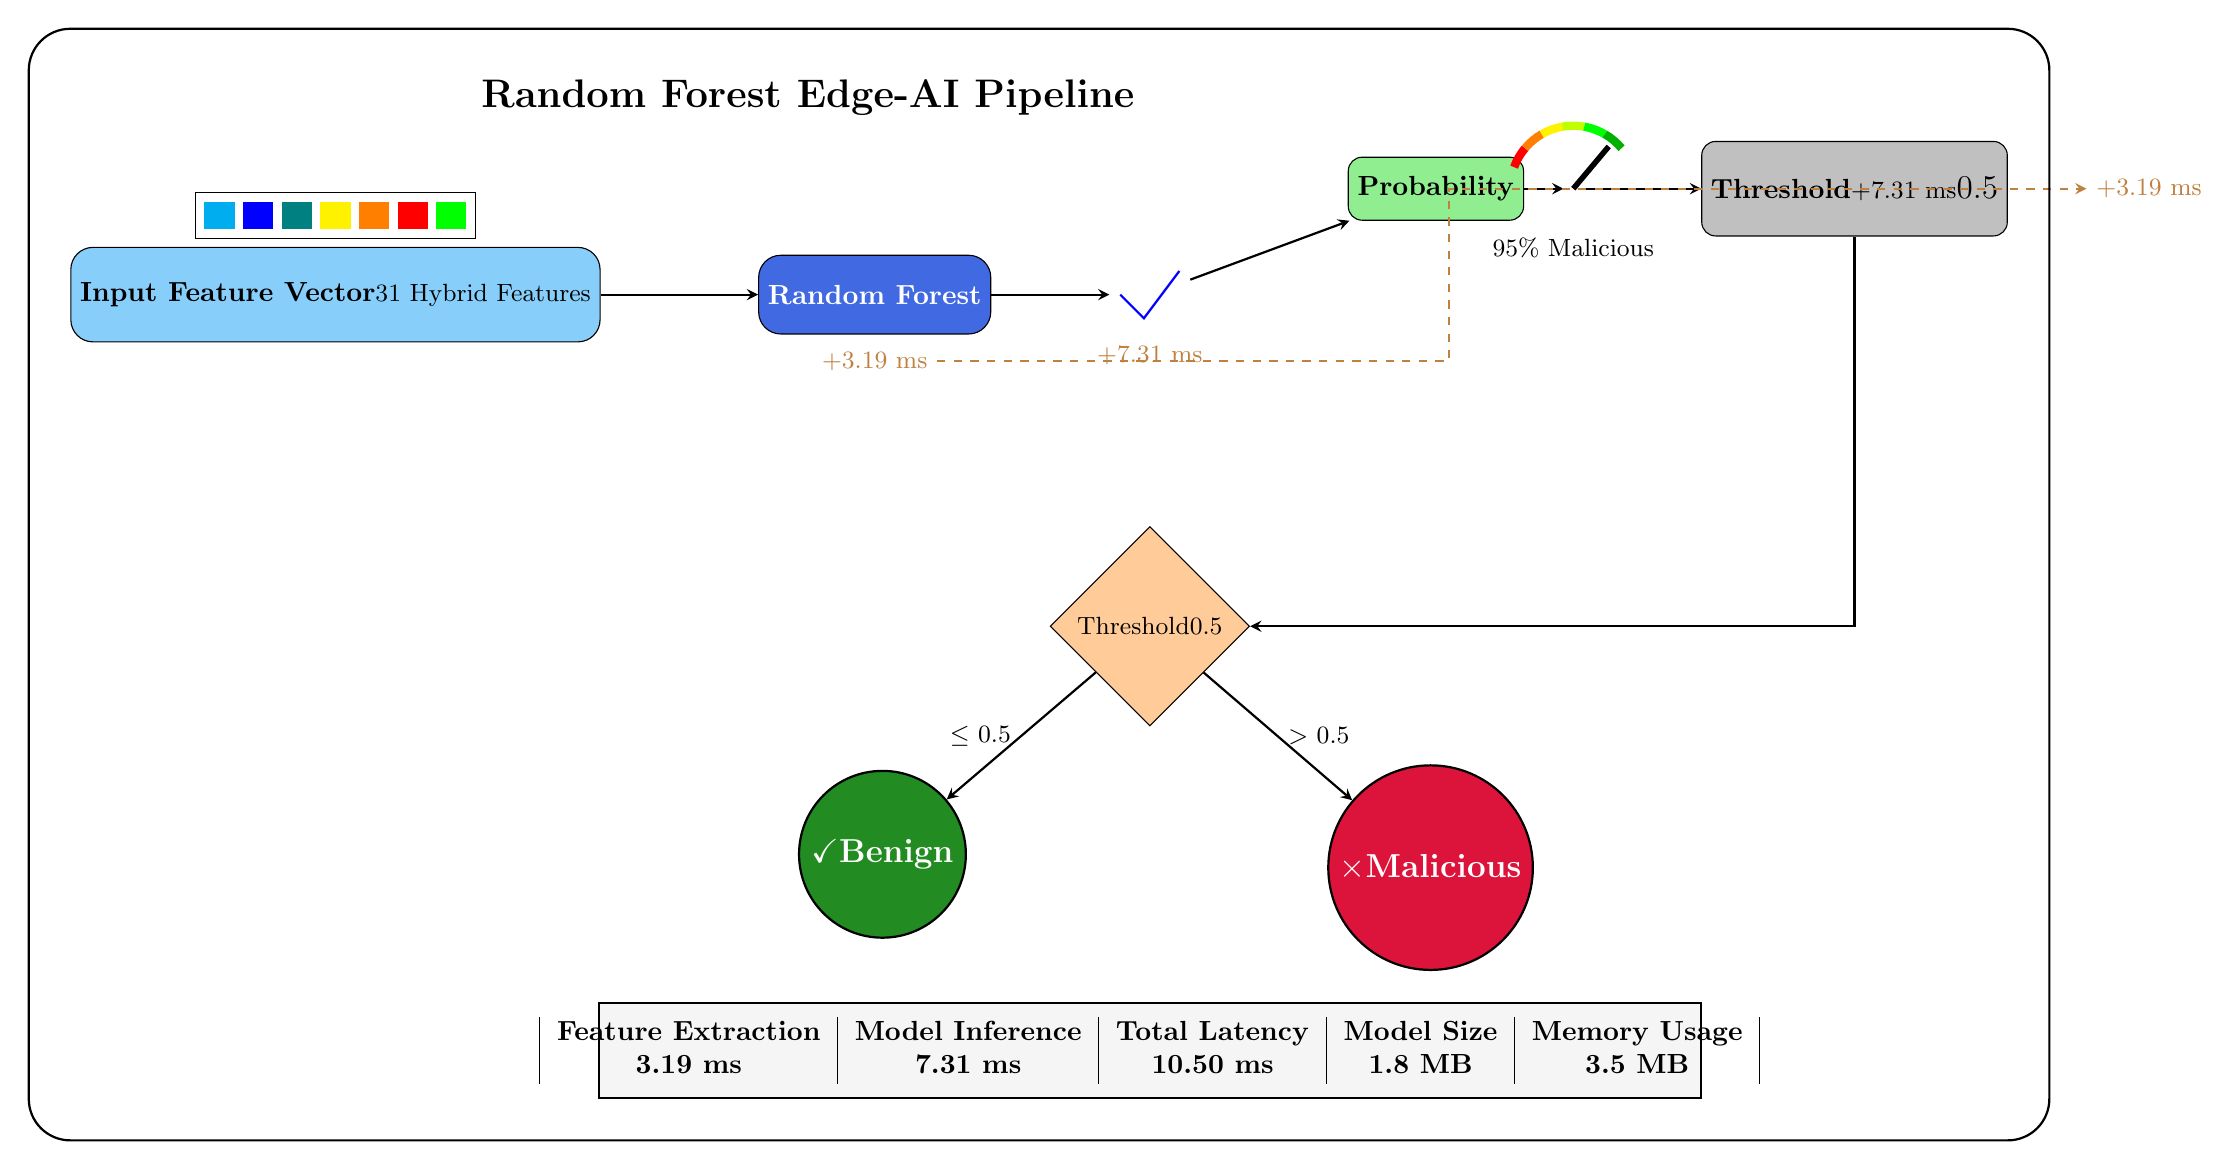
\begin{tikzpicture}[node distance=1.5cm]

% Title
\node[font=\Large\bfseries] (title) at (0,4.5) {Random Forest Edge-AI Pipeline};

% Input Feature Vector (left side)
\node[inputbox] (input) at (-6,2) {
    \textbf{Input Feature Vector}\\
    \small 31 Hybrid Features
};

% Feature colors legend above input
\node[above=0.1cm of input, rectangle, draw=black, minimum width=3cm, minimum height=0.4cm, fill=white] (legend) {
    \small\colorbox{cyan}{\phantom{x}} \colorbox{blue}{\phantom{x}} \colorbox{teal}{\phantom{x}} \colorbox{yellow}{\phantom{x}} \colorbox{orange}{\phantom{x}} \colorbox{red}{\phantom{x}} \colorbox{green}{\phantom{x}}
};

% Random Forest box
\node[rfbox, right=2cm of input] (rf) {
    \textbf{Random Forest}
};

% Feature extraction timing below RF
\node[timing, below=0.1cm of rf] (fe_time) {+3.19 ms};

% Random Forest symbol (checkmark)
\node[right=1.5cm of rf] (rf_symbol) {
    \tikz[scale=1.5]{\draw[thick, blue] (0,0.2) -- (0.2,0) -- (0.5,0.4);}
};

% Model inference timing below symbol
\node[timing, below=0.1cm of rf_symbol] (mi_time) {+7.31 ms};

% Probability box and gauge (upper right area)
\node[probbox, above right=0.5cm and 2cm of rf_symbol] (prob) {
    \textbf{Probability}
};

% Probability gauge (semicircle)
\node[right=0.5cm of prob] (gauge_center) {};
\begin{scope}[shift={(gauge_center)}]
    % Draw colored semicircle gauge
    \draw[thick, red, line width=3pt] (160:0.8) arc (160:140:0.8);
    \draw[thick, orange, line width=3pt] (140:0.8) arc (140:120:0.8);
    \draw[thick, yellow, line width=3pt] (120:0.8) arc (120:100:0.8);
    \draw[thick, lime, line width=3pt] (100:0.8) arc (100:80:0.8);
    \draw[thick, green, line width=3pt] (80:0.8) arc (80:60:0.8);
    \draw[thick, green!70!black, line width=3pt] (60:0.8) arc (60:40:0.8);
    
    % Needle pointing to high probability (~95%)
    \draw[thick, black, line width=2pt] (0,0) -- (50:0.7);
    \node[below=0.5cm, font=\small] {95\% Malicious};
\end{scope}

% Threshold box (upper right)
\node[threshbox, right=1.5cm of gauge_center] (threshold) {
    \textbf{Threshold}\\
    \small +7.31 ms\\
    \large 0.5
};

% Threshold timing arrow
\node[timing, right=1cm of threshold] (thresh_time) {+3.19 ms};

% Decision diamond (center bottom)
\node[decision, below=2.5cm of rf_symbol] (decision) {
    \small Threshold\\
    \small 0.5
};

% Results circles
\node[benign, below left=1.5cm and 2cm of decision] (benign_result) {
    \large $\checkmark$\\
    \textbf{Benign}
};

\node[malicious, below right=1.5cm and 2cm of decision] (malicious_result) {
    \large $\times$\\
    \textbf{Malicious}
};

% Main flow arrows
\draw[arrow] (input) -- (rf);
\draw[arrow] (rf) -- (rf_symbol);
\draw[arrow] (rf_symbol) -- (prob);
\draw[arrow] (prob) -- (gauge_center);
\draw[arrow] (gauge_center) -- (threshold);
\draw[arrow] (threshold) |- (decision);

% Decision arrows with labels
\draw[arrow] (decision) -- node[left, font=\small] {$\leq$ 0.5} (benign_result);
\draw[arrow] (decision) -- node[right, font=\small] {$>$ 0.5} (malicious_result);

% Dashed timing arrows
\draw[dashedarrow] (fe_time.east) -- ++(6.5,0) |- (thresh_time.west);

% Bottom performance metrics table
\node[below=3.5cm of decision, rectangle, draw=black, thick, minimum width=14cm, minimum height=1.2cm, fill=lightgray] (metrics) {};

\node[at=(metrics.center)] {
    \begin{tabular}{|c|c|c|c|c|}
    \textbf{Feature Extraction} & \textbf{Model Inference} & \textbf{Total Latency} & \textbf{Model Size} & \textbf{Memory Usage} \\
    \textbf{3.19 ms} & \textbf{7.31 ms} & \textbf{10.50 ms} & \textbf{1.8 MB} & \textbf{3.5 MB} \\
    \end{tabular}
};

% Main bounding box
\node[draw=black, thick, rounded corners=15pt, fit=(title)(legend)(input)(threshold)(benign_result)(malicious_result)(metrics), inner sep=15pt] (mainframe) {};

\end{tikzpicture}
\end{document}